\subsection*{Querying data}
DataJoint provides a minimal yet powerful set of operators on relations: restriction, projection, and join.
These operators allow transforming relations into new derived relations. 
Table \ref{algebra} summarizes these operators.

\begin{table*}
\begin{boxedminipage}{\textwidth}
\section*{Relational algebra}

Relational operators operate on existing relations to produce \emph{derived} relations for answering a wide variety of specific queries.
These operators do not retrieve any data from the database until the resulting expression is used to \emph{fetch} the data.
Relational operators are based on the concept of \emph{matching tuples}: 
Two tuples are considered matching  \emph{unless} they share an attribute with the same name but different values.

\subsection*{Restriction:  {\sf A \& B}, {\sf A -- B}}
The restriction A\&B denotes a relation comprising all tuples from A that match any tuple in {\sf B}.  

\begin{center}
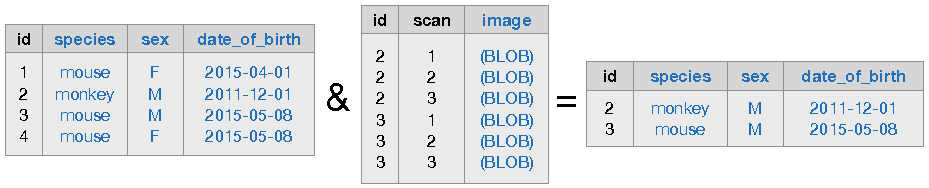
\includegraphics{./figures/restriction.pdf}
\end{center}

The inverse restriction {\sf A--B} denotes all tuples from {\sf A} that do not match any tuple in {\sf B}.

\begin{center}
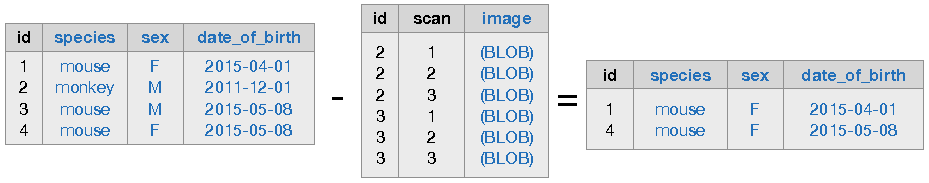
\includegraphics{./figures/antijoin.pdf}
\end{center}


\subsection*{Join: {\sf A * B}}
The join {\sf A*B} is the set of all tuples that can be produced by merging matching tuples from {\sf A} and {\sf B}:

\begin{center}
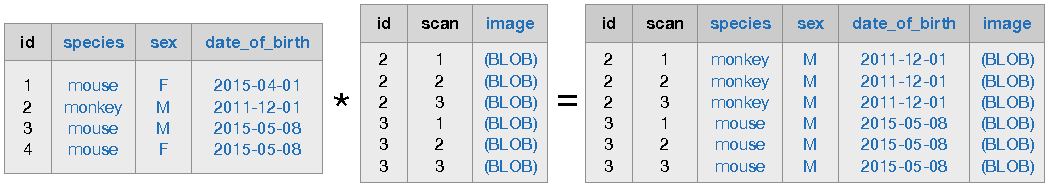
\includegraphics{./figures/join.pdf}
\end{center}
All attributes in {\sf A} and {\sf B} that share the same names must belong to the primary key in either relation.

\subsection*{Projection: {\sf A.pro(attributes)}}
The projection {\sf A.pro(attributes)} modifies the heading of {\sf A} by selecting a subset of its attributes (project), renaming attributes (rename), computing new attributes (expand), and computing summary statistics from other relations (aggregate).
The primary key attributes cannot be excluded from the resulting relation but may be renamed. 

\begin{center}
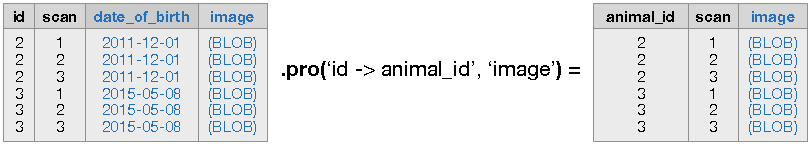
\includegraphics{./figures/project.pdf}
\end{center}

Please refer to the online documentation for more detailed descriptions.
\end{boxedminipage}
\caption{Relational operators of DataJoint}
\label{algebra}
\end{table*}


The output of each relational operator is a proper relation in its own right with its primary key, uniquely named attributes, and the full range of data query methods.
This property, called \emph{algebraic closure}, allows expressings highly specific queries from existing queries intuitively and laconically.

The starting point of any relational expression are base relations represented by their classes. 
For example, after executing the following assignment in either Python or MATLAB,
\mint{matlab}|rel = Ephys()|
the variable \matlab{rel} will represent the contents of the base relation \matlab{Ephys}, which represents electrophysiological recordings: local field potentials and spikes in our schema  (Fig.\ \ref{schema}\,B).

Restriction (represented by the logical AND operator {\tt \&}) selects a subset of tuples based on some condition.
For example, \matlab{Animal} may be restricted by a structure specifying values of attributes \matlab{species} and \matlab{sex},
in MATLAB,
\begin{minted}{matlab}
r.species = 'mouse'
r.sex = 'M'
\end{minted}
or in Python
\begin{minted}{python}
r = dict(species='mouse', sex='M')
\end{minted}
to produce the relation containing all male mice,
\mint{matlab}|male_mice = Animal() & r|

Relations can be restricted by conditions in the form of character strings, structures or structure arrays, or other relations.
For example, other relations may be restricted with \matlab{male_mice} even in combination with other restrictions:
\mint{matlab}|rel = Ephys() & male_mice & 'sampling_rate > 10000'|
The result \matlab{rel} will represent all Ephys recordings from male mice with acquisition sampling rates above 10 kHz when \matlab{sampling_rate} is an attribute of \matlab{Ephys}.


As another example, the relation \matlab{Running} contains episodes of the animals' locomotion inferred from treadmill sensor recordings in relation \matlab{Treadmill}.
Then the restriction
\mint{matlab}|rel = Session() & Running()|
represents all sessions with at least one episode of running.

Restrictions can also take the negative form using the \matlab{-} (minus) operator. For example,
\mint{matlab}|rel = (LFP() & Treadmill()) - Running()|
contains all LFP recordings in sessions that included treadmill recordings but no running episodes where found.

The join operator (\matlab{*}) produces a relation comprising all possible combinations of matching tuples from its two argument relations.

For example, the relation
\mint{matlab}|rel = Spikes() * LFP()|
will contain both spiking and LFP data for the same \matlab{Ephys} recordings.

Relational operators can be combined to produce highly specific expressions.  
For example,
\begin{minted}{matlab}
rel = Spikes() * LFP() & (Animal() * Session() & 
   'datediff(session_date, date_of_birth)<=28')
\end{minted}
is similar to the previous example but the result is restricted to cases when the animals were 28 days old or younger at the start of the recording session.
Since DataJoint passes its restriction conditions to SQL, restrictions can call SQL functions such as \matlab{datediff} here for computing the difference between the dates. 
Note that \matlab{session_date} comes from \matlab{Session} whereas \matlab{date_of_birth} comes from \matlab{Animal}. 
Thus the relation \matlab{Animal*Session} has both dates required for calculating the age. 

The \emph{projection} operator allows selecting and renaming attributes as well as computing new attributes, including summary statistics on other relations.  Please refer to the online documentation for additional details.

Relation objects are only symbolic representations of the data and relational expressions are only symbolic manipulations.
Once the desired relation is formulated, the actual data are retrieved from the database into a structure array using the \matlab{fetch} method
\mint{matlab}|data = rel.fetch()|
